\documentclass[a4paper,oneside,11pt]{scrartcl}
\usepackage[left=2cm,right=2cm,top=2.0cm,bottom=2.5cm,includeheadfoot]{geometry}
\usepackage[utf8]{inputenc}  % Replace "utf8" by "latin1" if your editor sucks.
\usepackage{fancyhdr}        % Better header and footer support.
\usepackage{titlesec}        % Alternative section titles.
\usepackage{amssymb}         % Math support.
\usepackage{amsmath}         % Math declarations.

% GraphViz support
\usepackage{graphicx}
\usepackage[x11names, rgb]{xcolor}
\usepackage{tikz}            % Drawing shapes.
\usepackage{caption}         % Captions for graphviz figures.
\usetikzlibrary{snakes,arrows,shapes}
\newcommand{\mygraph}[2]{%
  \vspace{1em}
  \includegraphics[width=15cm]{figures/#1.png}
  \captionof{figure}{#2}
  \vspace{1em}
}

% Variables.
% This file is automatically generated; do not edit
\newcommand{\productversion}{0.9.13 }

\newcommand{\productname}{Exscript}
\newcommand{\product}{{\it \productname} }

% Make references clickable.
\usepackage[colorlinks,hyperindex]{hyperref}
\hypersetup{%
  pdftitle    = {\productname\ Version \productversion},
  pdfkeywords = {exscript handbook telnet ssh python},
  pdfauthor   = {Samuel Abels},
  colorlinks  = true,
  %linkcolor   = blue,
}

% Initialize headers and footers.
\pagestyle{fancy}            % Use fancyhdr to render page headers/footers.
\fancyhf{}                   % Clear out old header/footer definition.

% Header
%\fancyhead[C]{\bfseries \productname}
\fancyhead[L]{\leftmark}
\fancyhead[R]{\MakeUppercase{\rightmark}}
\renewcommand{\headrulewidth}{0.5pt}

% Footer
\fancyfoot[C]{Page \thepage}
\renewcommand{\footrulewidth}{0.5pt}

% Enumerate using letters.
%\renewcommand{\labelenumi}{\alph{enumi})}

% Set source code options.
\usepackage{listings}
\lstset{language=python}
\lstset{commentstyle=\textit}
\lstset{showstringspaces=false}
\lstset{aboveskip=.1in,belowskip=.1in,xleftmargin=2em,basewidth=5pt}

% Do not indent paragraphs.
\parindent=0em

% Preformatted, indented text.
\usepackage{verbatim}
\makeatletter
\newenvironment{indentverb}
  {\def\verbatim@processline{%
  \hspace*{2em}\the\verbatim@line\par}%
  \verbatim}
  {\endverbatim}
\makeatother

% Title
\title{\productname\ Release \productversion\\
User Documentation\\
\vspace{5 mm}
\large A scripting language and framework for terminal based protocols}

% Hint boxes.
\usepackage{color}
\definecolor{nb}{gray}{.90}
\newcommand{\hint}[1]{
  \begin{center}
  \colorbox{nb}{
    \begin{tabular}{ll}
      \Large ! &
      \begin{minipage}{.92\linewidth}{
        \vspace{2mm}
        \sf #1
        \vspace{2mm}
      }\end{minipage}
    \end{tabular}
  }
  \end{center}
}

%
% Below comes the epydoc API boilerplate.
%
\usepackage{alltt, parskip, fancyhdr, boxedminipage}
\usepackage{makeidx, multirow, longtable, tocbibind, amssymb}
% Prompt
\newcommand{\pysrcprompt}[1]{\textcolor{py@ps1colour}{\small\textbf{#1}}}
\newcommand{\pysrcmore}[1]{\textcolor{py@ps2colour}{\small\textbf{#1}}}
% Source code
\newcommand{\pysrckeyword}[1]{\textcolor{py@keywordcolour}{\small\textbf{#1}}}
\newcommand{\pysrcbuiltin}[1]{\textcolor{py@builtincolour}{\small\textbf{#1}}}
\newcommand{\pysrcstring}[1]{\textcolor{py@stringcolour}{\small\textbf{#1}}}
\newcommand{\pysrcdefname}[1]{\textcolor{py@defnamecolour}{\small\textbf{#1}}}
\newcommand{\pysrcother}[1]{\small\textbf{#1}}
% Comments
\newcommand{\pysrccomment}[1]{\textcolor{py@commentcolour}{\small\textbf{#1}}}
% Output
\newcommand{\pysrcoutput}[1]{\textcolor{py@outputcolour}{\small\textbf{#1}}}
% Exceptions
\newcommand{\pysrcexcept}[1]{\textcolor{py@exceptcolour}{\small\textbf{#1}}}
\newlength{\funcindent}
\newlength{\funcwidth}
\setlength{\funcindent}{1cm}
\setlength{\funcwidth}{\textwidth}
\addtolength{\funcwidth}{-2\funcindent}
\newlength{\varindent}
\newlength{\varnamewidth}
\newlength{\vardescrwidth}
\newlength{\varwidth}
\setlength{\varindent}{1cm}
\setlength{\varnamewidth}{.3\textwidth}
\setlength{\varwidth}{\textwidth}
\addtolength{\varwidth}{-4\tabcolsep}
\addtolength{\varwidth}{-3\arrayrulewidth}
\addtolength{\varwidth}{-2\varindent}
\setlength{\vardescrwidth}{\varwidth}
\addtolength{\vardescrwidth}{-\varnamewidth}
\newenvironment{Ventry}[1]%
 {\begin{list}{}{%
   \renewcommand{\makelabel}[1]{\texttt{##1:}\hfil}%
   \settowidth{\labelwidth}{\texttt{#1:}}%
   \setlength{\leftmargin}{\labelsep}%
   \addtolength{\leftmargin}{\labelwidth}}}%
 {\end{list}}
\usepackage[utf8]{inputenc}
\definecolor{UrlColor}{rgb}{0,0.08,0.45}
   % Import common styles.
\fancyfoot[C]{Page \thepage}
\title{\productname\ Release \productversion\\
User Documentation\\
\vspace{5 mm}
\large A scripting language and framework for terminal based protocols}
\author{Samuel Abels}

\begin{document}
\maketitle
\tableofcontents

\newpage
\section{Introduction}
\subsection{Why \productname?}

\product is a script and template language for automating network connections 
over protocols such as Telnet or SSH. \product is targeted at non-developers 
and developers alike.

\product is often used to automate sessions with routers from Cisco, Juniper, 
Huawei, and others. It may be used by an administrator who often configures 
machines running Linux/Unix, IOS, IOS-XR, JunOS, VRP, or any other operating 
system that can be used with a terminal.

\product is in some ways comparable to Expect, but has some unique features 
that make it a lot easier to use and understand for non-developers. 


\subsection{Legal Information}

\product and this handbook are distributed under the terms and conditions 
of the GNU GPL (General Public License) Version 2. You should have received 
a copy of the GPL along with \product. If you did not, you may read it here:

\vspace{1em}
\url{http://www.gnu.org/licenses/gpl-2.0.txt}
\vspace{1em}

If this license does not meet your requirements you may contact us under 
the points of contact listed in the following section. Please let us know 
why you need a different license - perhaps we may work out a solution 
that works for either of us.


\subsection{Contact Information \& Feedback}

If you spot any errors, or have ideas for improving \product or this 
documentation, your suggestions are gladly accepted.
We offer the following contact options: \\

\begin{tabular}{ll}
{\bf Google Groups:} & http://groups.google.com/group/exscript/ \\
{\bf Phone:}         & +49 176 830 40288 \\
{\bf Jabber:}        & knipknap@jabber.org
\end{tabular}


\newpage
\section{Overview}
\subsection{Quick Introduction}

With \product you can quickly automate a conversation with a device over 
Telnet or SSH. For example, to execute the ``ls'' command on three different 
hosts, create a file with the following content: 

\begin{lstlisting}
ls
\end{lstlisting}

and then run it using

\begin{lstlisting}
exscript my_template host1 host2 host3
\end{lstlisting}


\subsection{Talking To Multiple Devices At The Same Time}

With \product you can automatically parallelize your connections, such that 
multiple sessions are opened at the same time. This can speed up the time 
in which a specific command is propagated within your network.

For example, imagine you want to execute the ``clear ip bgp * soft'' 
command on twenty different Cisco routers. Start by creating a text file 
with the following content: 

\begin{lstlisting}
clear ip bgp * soft
\end{lstlisting}

Save this file as commands.exscript. Also, create a text file that contains 
the list of hostnames to which the command should be sent: 

\begin{lstlisting}
host1
host2
...
host20
\end{lstlisting}

Save this file as hosts.txt. To send this change to all routers at the same 
time, type the following command: 

\begin{lstlisting}
exscript --hosts hosts.txt -c15 commands.exscript
\end{lstlisting}

Note that the -c15 option causes \product to open a maximum of fifteen 
connections at the same time. Once the first host out of these 15 is 
completed, \product opens the connection to the next host, until the 
``clear ip bgp * soft'' command has been sent to all hosts. 


\subsection{Advanced Command Templates}

\product templates support many more commands. For example, to automate a 
session with a Cisco router, the following template may be used: 

\begin{lstlisting}
show version {extract /^(cisco)/ as vendor}
{if vendor is "cisco"}
  show ip interface brief {extract /^(\S+)\s/ as interfaces}
  {loop interfaces as interface}
    show running interface $interface
    configure terminal
    interface $interface
    no shut
    end
  {end}
  copy running-config startup-config
{end}
\end{lstlisting}

\product provides additional methods for interacting with the remote 
host and for receiving information from it.
The following chapters include a more complete overview of the template 
language.


\section{Command Line Syntax}
\subsection{Overview}

You can pass parameters (or lists of parameters) into the templates and 
use them to drive what happens on the remote host. \product easily supports 
logging, authentication mechanisms such as TACACS and takes care of 
synchronizing the login procedure between multiple running connections.

These features are enabled using simple command line options. The following 
options are currently provided:

% This file is automatically generated; do not edit
\begin{lstlisting}
Syntax: exscript [options] exscript [hostname [hostname ...]]
  -c, --connections NUM
                 Maximum number of concurrent connections.
                 NUM is a number between 1 and 20, default is 1
      --csv-hosts FILE
                 Loads a list of hostnames and definitions from the given file.
                 The first line of the file must have the column headers in the
                 following syntax:
                    hostname [variable] [variable] ...
                 where the fields are separated by tabs, "hostname" is the
                 keyword "hostname" and "variable" is a unique name under
                 which the column is accessed in the script.
                 The following lines contain the hostname in the first column,
                 and the values of the variables in the following columns.
  -d, --define PAIR
                 Defines a variable that is passed to the script.
                 PAIR has the following syntax: <STRING>=<STRING>.
      --default-domain STRING
                 The IP domain name that is used if a given hostname has no 
                 domain appended.
      --hosts FILE
                 Loads a list of hostnames from the given file (one host per
                 line).
  -i, --non-interactive
                 Do not ask for a username or password.
  -l, --logdir DIR
                 Logs any communication into the directory with the given name.
                 Each filename consists of the hostname with "_log" appended.
                 Errors are written to a separate file, where the filename
                 consists of the hostname with ".log.error" appended.
      --no-echo
                 Turns off the echo, such that the network activity is no longer
                 written to stdout.
                 This is already the default behavior if the -c option was given
                 with a number greater than 1.
      --overwrite-logs
                 Instructs Exscript to overwrite existing logfiles. The default
                 is to append the output if a log already exists.
  -n, --no-authentication
                 When given, the authentication procedure is skipped. Implies -i.
      --no-auto-logout
                 Do not attempt to execute the exit or quit command at the end
                 of a script.
      --no-prompt
                 Do not wait for a prompt anywhere. Note that this will also
                 cause Exscript to disable commands that require a prompt, such
                 as 'extract'.
      --no-initial-prompt
                 Do not wait for a prompt after sending the password.
  -p, --protocol STRING
                 Specify which protocol to use to connect to the remote host.
                 STRING is one of: telnet ssh
                 The default protocol is telnet.
      --sleep TIME
                 Waits for the specified time before running the script.
                 TIME is a timespec as specified by the 'sleep' Unix command.
      --ssh-auto-verify
                 Automatically confirms the 'Host key changed' SSH error 
                 message with 'yes'. Highly insecure and not recommended.
      --ssh-key FILE
                 Specify a key file that is passed to the SSH client.
                 This is equivalent to using the -i parameter with ssh.
  -v, --verbose NUM
                 Print out debug information about the network activity.
                 NUM is a number between 0 (min) and 5 (max)
  -V, --parser-verbose NUM
                 Print out debug information about the Exscript parser.
                 NUM is a number between 0 (min) and 5 (max)
      --version  Prints the version number.
  -h, --help     Prints this help.
\end{lstlisting}



\subsection{Using Account Pooling}

It is possible to provide an account pool from which Exscript takes a 
user account whenever it needs to log into a remote host. Depending on 
the authentification mechanism used in your network, you may significantly 
increase the speed of parallel connections by using more than one account 
in parallel. The following steps need to be taken to use the feature:

\begin{enumerate}
\item Create a file with the following format:

\begin{lstlisting}
[account-pool]
user=password
other_user=another_password
somebody=yet_another_password
\end{lstlisting}

Note that the password needs to be base64 encrypted, just putting plain
passwords there will NOT work.

\item Save the file. It is assumed that you are aware of the security 
implications of saving your login passwords in a text file.
\item Start Exscript with the "--account-pool FILE" option. For example:

\begin{lstlisting}
exscript --account-pool /home/user/my_accounts my.exscript host4
\end{lstlisting}
\end{enumerate}


\subsection{Using a CSV file as input}

By providing the --csv-hosts option you may pass a list of hosts to 
Exscript while at the same time providing a number of variables to 
the script. The CSV file should have the following format: 

\begin{lstlisting}
hostname my_variable another_variable
myhost value another_value
yourhost hello world
\end{lstlisting}

Note that fields are separated using the tab character, and the first 
line must start with the string "hostname" and is followed by a list of 
column names.

In the Exscript, you may then access the variables using those column names: 

\begin{lstlisting}
ls -l $my_variable
touch $another_variable
\end{lstlisting}


\section{Language Syntax}
\subsection{Sending Commands To The Remote Host}

The simplest possible template is one that contains only the commands 
that are sent to the remote host. For example, the following \product 
can be used to retrieve the response of the ls -l and df commands from 
a unix host: 

\begin{lstlisting}
ls -l
df
\end{lstlisting}

Save this file as ``my.exscript'' and execute it using the following 
command: 

\begin{lstlisting}
exscript my.exscript localhost 
\end{lstlisting}

where ``localhost'' is the name of the host on which the ``ls -l'' 
and ``df'' commands are executed. 


\subsection{Comments}

Lines starting with a hash (``\#'') are interpreted as comments and ignored. 
For example: 

\begin{lstlisting}
1. # This line is ignored...
2. {if __hostname__ is "test"}
3.   # ...and so is this one.
4. {end}
\end{lstlisting}


\subsection{Using Variables}

The following template uses a variable to execute the ls command with a 
filename as an argument: 

\begin{lstlisting}
ls -l $filename
\end{lstlisting}

Execute:

\begin{lstlisting}
exscript -d filename=.profile my.exscript localhost 
\end{lstlisting}

Note that the -d switch allows passing variables into the \product. The 
example executes the command ls -l .profile. 
You can also assign a value to a variable within an \product: 

\begin{lstlisting}
{filename = ".profile"}
ls -l $filename
\end{lstlisting}

You may also use variables in strings by prefixing them with the ``\$'' 
character: 

\begin{lstlisting}
1. {test = "my test"}
2. {if "my test one" is "$test one"}
3.   # This matches!
4. {end}
\end{lstlisting}

In the above template line 3 is reached. If you don't want the ``\$'' 
character to be interpreted as a variable, you may prefix it with a 
backslash: 

\begin{lstlisting}
1. {test = "my test"}
2. {if "my test one" is "\$test one"}
3.   # This does not match
4. {end}
\end{lstlisting}

\subsection{Adding Variables To A List}

In \product every variable is a list. You can also merge two lists by 
using the ``append'' keyword: 

\begin{lstlisting}
1. {
2.   test1 = "one"
3.   test2 = "two"
4.   append test2 to test1
5. }
\end{lstlisting}

This results in the ``test1'' variable containing two items, ``one'' and 
``two''.

\subsection{Using Built-in Variables}

The following variables are available in any \product template, even if 
they were not explicitly passed in:

\begin{enumerate}
\item {\bf \_\_hostname\_\_} contains the hostname that was used to open the 
current connection.
\item {\bf \_\_response\_\_} contains the response of the remote host that was 
received after the execution of the last command. 
\end{enumerate}

Built-in variables are used just like any other variable. You can also 
assign a new value to a built-in variable in the same way. 


\subsection{Using Expressions}

An expression is a combination of values, variables, operators, and functions 
that are interpreted (evaluated) according to particular rules and that 
produce a return value. For example, the following code is an expression:

\begin{lstlisting}
name is "samuel" and 4 * 3 is not 11
\end{lstlisting}

In this expression, {\it name} is a variable, {\it is}, {\it is not}, and 
{\it *} are operators, and {\it "samuel"}, {\it 4}, {\it 3}, and {\it 11} 
are values. The return value of this particular expression is {\it true}.

In \product, expressions are used in many places, such as if-conditions or 
variable assignments. The following operators may be used in an expression. 


\subsubsection{Priority 1 Operators}

\begin{enumerate}
\item {\it *} multiplies the operators (numerically).
\item {\it /} divides the operators (numerically).
\end{enumerate}


\subsubsection{Priority 2 Operators}

\begin{enumerate}
\item {\it +} adds the operators (numerically). 
\item {\it -} subtracts the operators (numerically). 
\end{enumerate}


\subsubsection{Priority 3 Operators}

\begin{enumerate}
\item {\it .} concatenates two strings.
\end{enumerate}


\subsubsection{Priority 4 Operators}

\begin{enumerate}
\item {\it is} tests for equality. If both operators are lists, only the 
first item in the list is compared.
\item {\it is not} produces the opposite result from is.
\item {\it in} tests whether the left string equals any of the items in the 
list given as the right operator.
\item {\it not in} produces the opposite result from in.
\item {\it matches} tests whether the left operator matches the regular 
expression that is given as the right operator. 
\item {\it ge} tests whether the left operator is (numerically) greater than 
or equal to the right operator. 
\item {\it gt} tests whether the left operator is (numerically) greater than 
the right operator. 
\item {\it le} tests whether the left operator is (numerically) less than or 
equal to the right operator. 
\item {\it lt} tests whether the left operator is (numerically) less than the 
right operator. 
\end{enumerate}


\subsubsection{Priority 5 Operators}

\begin{enumerate}
\item {\it not} inverts the result of a comparison. 
\end{enumerate}


\subsubsection{Priority 6 Operators}

\begin{enumerate}
\item {\it and} combines two tests such that a logical AND comparison is made. 
If the left operator returns FALSE, the right operator is not evaluated.
\item {\it or} combines two tests such that a logical OR comparison is made. 
If the left operator returns TRUE, the right operator is not evaluated. 
\end{enumerate}


\subsection{Using Hexadecimal Or Octal Numbers}

\product also supports hexadecimal and octal numbers using the following 
syntax: 

\begin{lstlisting}
{
  if 0x0a is 012
    sys.message("Yes")
  else
    sys.message("No")
  end
}
\end{lstlisting}


\subsection{Using Regular Expressions}

At some places \product uses Regular Expressions. These are NOT the same as 
the expressions documented above, and if you do not know what regular 
expressions are it is recommended that you read a tutorial on regular 
expressions first.

\product regular expressions are similar to Perl and you may also append 
regular expression modifiers to them. For example, the following is a valid 
regular expression in \product: 

\begin{lstlisting}
/^cisco \d+\s+\w/i
\end{lstlisting}

Where the appended ``i'' is a modifier (meaning case-insensitive). A full 
explanation of regular expressions is not given here, because plenty of 
introductions have been written already and may be found with the internet 
search engine of your choice.


\section{\product Commands}

By default, any content of an \product is sent to the remote host. However, 
you can also add instructions with special meanings. Such instructions are 
enclosed by curly brackets ({ and }). The following commands all use this 
syntax. 

\subsection{Extracting Data From A Response}

\product lets you parse the response of a remote host using regular 
expressions. If you do not know what regular expressions are, please read 
a tutorial on regular expressions first.

\subsubsection{extract ... into ...}

If you already know what regular expressions are, consider the following 
template: 

\begin{lstlisting}
ls -l {extract /^(d.*)/ into directories}
\end{lstlisting}

The extract command matches each line of the response of ``ls -l'' against 
the regular expression /\^(d.*)/ and then appends the result of the first 
match group (a match group is a part of a regular expression that is 
enclosed by brackets) to the list variable named directories. 

You can also extract the value of multiple match groups using the following 
syntax: 

\begin{lstlisting}
ls -l {extract /^(d\S+)\s.*\s(\S+)$/ into modes, directories}
\end{lstlisting}

This extracts the mode and the directory name from each line and appends 
them to the modes and directories lists respectively. You can also apply 
multiple matches to the same response using the following syntax: 

\begin{lstlisting}
ls -l {
  extract /^[^d].*\s(\S+)$/ into files
  extract /^d.*\s(\S+)$/    into directories
}
\end{lstlisting}

There is no limit to the number of extract statements. 


\subsubsection{extract ... into ... from ...}

When used without the ``from'' keyword, ``extract'' gets the values from the 
last command that was executed. You may however also instruct \product to 
extract the values from a variable. The following example shows how this 
may be done. 

\begin{lstlisting}
ls -l {
  extract /^(.*)/  into lines
  extract /^(d.*)/ into directories from lines
}
\end{lstlisting}


\subsubsection{extract ... as ...}

The ``as'' keyword is similar to ``into'', the difference being that with 
as, the destination variable is cleared before new values are appended. 

\begin{lstlisting}
ls -l {extract /^(d.*)/ as directories}
\end{lstlisting}

``as'' may be used anywhere where ``into'' is used.


\subsection{Using If-Conditions}

You can execute commands depending on the runtime value of a variable or 
expression. 

\subsubsection{if ... end}

The following \product executes the ``ls'' command only if ``ls -l .profile'' 
did not produce a result: 

\begin{lstlisting}
ls -l .profile {extract /(\.profile)$/ as found}
{if found is not ".profile"}
  ls
{end}
\end{lstlisting}


\subsubsection{if ... else ... end}

You can also add an else condition: 

\begin{lstlisting}
ls -l .profile {extract /(\.profile)$/ as found}
{if found is not ".profile"}
  ls
{else}
  touch .profile
{end}
\end{lstlisting}


\subsubsection{if ... else if ...}

You can perform multiple matches using else if: 

\begin{lstlisting}
ls -l .profile {extract /(.*profile)$/ as found}
{if found is ".profile"}
  ls
{else if found matches /my_profile/}
  ls -l p*
{else}
  touch .profile
{end}
\end{lstlisting}


\subsection{Loops}

You can execute commands multiple times using the ``loop'' statement. The 
following \product executes the ``ls'' command three times: 

\begin{lstlisting}
{number = 0}
{loop until number is 3}
  {number = number + 1}
  ls $directory
{end}
\end{lstlisting}

Similarly, the while statement may be used. The following script is 
equivalent: 

\begin{lstlisting}
{number = 0}
{loop while number is not 3}
  {number = number + 1}
  ls $directory
{end}
\end{lstlisting}

Another alternative is using the ``loop from ... to ...'' syntax, which 
allows you to specify a range of integers: 

\begin{lstlisting}
# Implicit "counter" variable.
{loop from 1 to 3}
  ls $directory$counter
{end}

# Explicit variable name.
{loop from 1 to 3 as number}
  ls $directory$number
{end}
\end{lstlisting}


\subsection{Loops And Lists}

The following \product uses the ls command to show the content of a list 
of subdirectories: 

\begin{lstlisting}
ls -l {extract /^d.*\s(\S+)$/ as directories}
{loop directories as directory}
  ls $directory
{end}
\end{lstlisting}

You can also walk through multiple lists at once, as long as they have the 
same number of items in it: 

\begin{lstlisting}
ls -l {extract /^(d\S+)\s.*\s(\S+)$/ as modes, directories}
{loop modes, directories as mode, directory}
  echo Directory has the mode $mode
  ls $directory
{end}
\end{lstlisting}

List loops can also be combined with the until or while statement seen in 
the previous section: 

\begin{lstlisting}
ls -l {extract /^d.*\s(\S+)$/ as directories}
{loop directories as directory until directory is "my_subdir"}
  ls $directory
{end}
\end{lstlisting}


\subsection{Using Functions}

\product provides builtin functions with the following syntax: 

\begin{lstlisting}
type.function(EXPRESSION, [EXPRESSION, ...])
\end{lstlisting}

For example, the following function instructs \product to wait for 10 seconds: 

\begin{lstlisting}
{sys.wait(10)}
\end{lstlisting}

For a list of supported functions please refer to appendix \ref{stdlib}.


\subsection{Exiting A Script}

\subsubsection{fail ``message''}

The ``fail'' keyword may be used where a script should terminate immediately. 

\begin{lstlisting}
show something
{fail "Error: Failed!"}
show something else
\end{lstlisting}

In this script, the ``show something else'' line is never reached. 

\subsubsection{fail ``message'' if ...}

It is also possible to fail only if a specific condition is met. The 
following snippet terminates only if a Cisco router does not have a POS 
interface: 

\begin{lstlisting}
show ip int brie {
  extract /^(POS)\S+/ as pos_interfaces
  fail "No POS interface found!" if "POS" not in pos_interfaces
}
\end{lstlisting}


\subsection{Error Handling}

\product attempts to detect errors, such as commands that are not understood 
by the remote host. By default, \product considers any response that 
includes one of the following strings to be an error: 

\begin{lstlisting}
invalid
incomplete
unrecognized
unknown command
[^\r\n]+ not found
\end{lstlisting}

If this default configuration does not suit your needs, you can override the 
default, setting it to any regular expression of your choice using the 
following function: 

\begin{lstlisting}
{connection.set_error(/[Ff]ailed/)}
\end{lstlisting}

Whenever such an error is detected, the currently running \product is 
cancelled on the current host. For example, when the following script is 
executed on a Cisco router, it will fail because there is no ls command: 

\begin{lstlisting}
ls -l
show ip int brief
\end{lstlisting}

The ``show ip int brief'' command is not executed, because an error is 
detected at ``ls -l'' at runtime.

If you want to execute the command regardless, you can wrap the ``ls'' 
command in a ``try'' block: 

\begin{lstlisting}
{try}ls -l{end}
show ip int brief
\end{lstlisting}

You can add as many commands as you like in between a try block. For 
example, the following will also work: 

\begin{lstlisting}
{try}
  ls -l
  df
  show running-config
{end}
show ip int brief
\end{lstlisting}


\section{Trouble Shooting}
\subsection{Common Pitfalls}

Generally, the following kinds of errors that may happen at runtime:

\begin{enumerate}
\item {\bf A script deadlocks.} In other words, \product sends no further 
commands even though the remote host is already waiting for a command. 
This generally happens when a prompt is not recognized. 
\item {\bf A script executes a command before the remote host is ready.} 
This happens when a prompt was detected where none was really included 
in the response. 
\item {\bf A script terminates before executing all commands.} This 
happens when two (or more) prompts were detected where only one was 
expected. 
\end{enumerate}

The following sections explain when these problems may happen and how to fix them. 

\subsection{Deadlocks}

\product tries to automatically detect a prompt, so generally you should 
not have to worry about prompt recognition. The following prompt types 
are supported: 

\begin{lstlisting}
[sam123@home ~]$
sam@knip:~/Code/exscript$
sam@MyHost-X123$
MyHost-ABC-CDE123$
MyHost-A1$
MyHost-A1(config)$
FA/0/1/2/3$
FA/0/1/2/3(config)$
admin@s-x-a6.a.bc.de.fg:/$
\end{lstlisting}

Note: The trailing ``\$'' may also be any of the following characters: ``\$\#>\%''

However, in some rare cases, a remote host may have a prompt that \product 
can not recognize. Similarly, in some scripts you might want to execute a 
special command that triggers a response that does not include a prompt 
\product can recognize.

In both cases, the solution includes defining the prompt manually, such 
that \product knows when the remote host is ready. For example, consider 
the following script: 

\begin{lstlisting}
1. show ip int brief
2. write memory
3. {enter}
4. show configuration
\end{lstlisting}

Say that after executing line 2 of this script, the remote host asks for a 
confirmation, saying something like this: 

\begin{lstlisting}
Are you sure you want to overwrite the configuration? [confirm]
\end{lstlisting}

Because this answer does not contain a standard prompt, \product can not 
recognize it. We have a deadlock. To fix this, we must tell \product that 
a non-standard prompt should be expected. The following change fixes the 
script: 

\begin{lstlisting}
1. show ip int brief
2. {connection.set_prompt(/\[confirm\]/)}
3. write memory
4. {connection.set_prompt()}
5. {enter}
6. show configuration
\end{lstlisting}

The second line tells \product to wait for ``[confirm]'' after executing 
the following commands. Because of that, when the write memory command was 
executed in line 3, the script does not deadlock (because the remote host's 
response includes ``[confirm]''). In line 4, the prompt is reset to it's 
original value. This must be done, because otherwise the script would wait 
for another ``[confirm]'' after executing line 5 and line 6. 


\subsection{A Command Is Sent Too Soon}

This happens when a prompt was incorrectly detected in the response of a 
remote host. For example, consider using the following script:

\begin{lstlisting}
show interface descriptions{extract /^(\S+\d)/ as interfaces}
show diag summary
\end{lstlisting}

Using this script, the following conversation may take place:

\begin{lstlisting}
1. router> show interface descriptions
2. Interface              Status         Protocol Description
3. Lo0                    up             up       Description of my router>
4. PO0/0                  admin down     down     
5. Serial1/0              up             up       My WAN link
6. router> 
\end{lstlisting}

Note that line 3 happens to contain the string ``Router>'', which looks like 
a prompt when it really is just a description. So after receiving the ``>'' 
character in line 3, Exscript believes that the router is asking for the 
next command to be sent. So it immediately sends the next command (``show 
diag summary'') to the router, even that the next prompt was not yet received.

Note that this type of error may not immediately show, because the router may 
actually accept the command even though it was sent before a prompt was sent. 
It will lead to an offset however, and may lead to errors when trying to 
capture the response. It may also lead to the script terminating too early.

To fix this, make sure that the conversation with the remote host does 
not include any strings that are incorrectly recognized as prompts. You can 
do this by using the ``connection.set\_prompt(...)'' function as explained 
in the sections above.


\subsection{The Connection Is Closed Too Soon}

This is essentially the same problem as explained under ``A Command Is Sent 
Too Soon''. Whenever a prompt is (correctly or incorrectly) detected, 
the next command is send to the remote host.
If all commands were already executed and the next prompt is received (i.e. 
the end of the script was reached), the connection is closed.

To fix this, make sure that the conversation with the remote host does 
not include any strings that are incorrectly recognized as prompts. You can 
do this by using the ``connection.set\_prompt(...)'' function as explained 
in the sections above. 


\section{The Python API}
\subsection{Overview}

\product provides simple, yet powerful Python APIs. There are two ways in 
which \product APIs may be used:

\begin{enumerate}
\item ``\product.protocols'' is a simple replacement for Python's built-in 
telnetlib.
\item ``\product.Queue'' is a powerful, multi-threaded environment for 
automating more complex tasks. It comes with features such as logging, 
user account management, and error handling that make things a lot 
easier. This is the recommended way of using Exscript.
\end{enumerate}


\subsection{\product.protocols}

The telnetlib module shipped with Python is incomplete, poorly implemented, 
and does not feature a generic API. To make it easy to access hosts via 
Telnet and SSH using the exact same API, \product.protocols provides a 
clean and simple replacement.
\product supports the following protocols at this time:

\begin{enumerate}
\item {\it Telnet} is a Telnet adapter.
\item {\it SSH} is an adapter for SSH version 1 and version 2.
\item {\it Dummy} is a virtual pseudo device that may be used for testing.
\end{enumerate}

The following example shows how to connect to a host using Telnet:

\begin{lstlisting}
from Exscript.protocols import Telnet

conn = Telnet()
conn.connect("127.0.0.1") # The default port is 21
conn.authenticate("myuser", "mypassword")
conn.execute("ls -l")
conn.send("exit\r")
conn.close()
\end{lstlisting}

The example will execute the "ls -l" command on the remote host, and 
waits until the remote host has responded with a prompt.
Once the prompt was retrieved, the function returns and 
``conn.send("exit\r")'' is reached.
Unlike {\it execute()}, the {\it send()} method returns immediately without 
waiting for a response from the remote host. This is necessary here, because 
the remote host does not normally respond to the ``exit'' command; it just 
closes the connection.

The above code also works with SSH - just replace "Telnet" with SSH:

\begin{lstlisting}
from Exscript.protocols import SSH
conn = SSH()
...
\end{lstlisting}

To fetch the response of a remote host, the following code may be used:

\begin{lstlisting}
...
conn.execute("ls -l")
print "The host said:", repr(conn.response)
\end{lstlisting}


\subsubsection{Emulating A Remote Device}

\product also provides a dummy protocol adapter for testing 
purposes. It emulates a remote host and may be used in place of the Telnet 
and SSH adapters:

\begin{lstlisting}
from Exscript.protocols import Dummy
conn = Dummy()
...
\end{lstlisting}

In order to define the behavior of the dummy, you may define it by 
providing a Python file that maps commands to responses. E.g.:

\begin{lstlisting}
def echo(command):
    return command.split(' ', 1)[1]

commands = (
('ls -l', """
-rw-r--r-- 1 sab nmc 1906 Oct  5 11:18 Makefile
-rw-r--r-- 1 sab nmc 1906 Oct  5 11:18 myfile
"""),

(r'echo [\r\n]+', echo)
)
\end{lstlisting}

Note that the command name is a regular expression, and the response may 
be either a string or a function.


\subsection{\product.Queue}

The more powerful and recommended way of using Exscript is by using 
\product.Queue.
Consider the following simple example:

\lstinputlisting{../demos/simple/simple.py}

This code reads a list of hostnames from ``hostlist.txt'', automatically
logs into each of the hosts, and executes the ``do\_something'' once
for each of the hosts.

The ``quickstart()'' function is a shortcut that you can use in most cases.
However, there are some more advanced features that you can use. For
example, Exscript can generate a report for all of the executed tasks:

\lstinputlisting{../demos/report/report.py}

\product provides additional methods, and also offers protocol-specific 
options. For a complete list of supported methods please refer to our API 
documentation.


\newpage
\section{The Exscript Server}
\subsection{Overview}

The \product daemon is a server that takes an order and runs services
asynchronously. It may, for example, be used as a backend for running
\product through a web server.

Prerequisite: \product is already installed and working.

The \product daemon is built provides services to an external caller,
and runs one or more instances of Exscript internally. Here is a
general overview:

\includegraphics{exscript-architecture}


\subsection{Installation}

The following instructions should work on most Debian based Linux
distributions. On other systems the procedure will probably differ.

\begin{enumerate}
\item Define the directories for the following steps:

\begin{verbatim}
    export EXSCRIPT_LOG=/var/log/exscriptd
    export EXSCRIPT_SPOOL=/var/spool/exscriptd
    export EXSCRIPT_CFG=/etc/exscriptd
    export EXSCRIPT_USER=exscriptd
    export EXSCRIPT_GROUP=exscriptd
\end{verbatim}

\item Create a user and group for the daemon:

\begin{verbatim}
    sudo adduser $EXSCRIPT_USER $EXSCRIPT_GROUP
\end{verbatim}

\item Create the required directories:

\begin{verbatim}
    sudo mkdir -p $EXSCRIPT_LOG $EXSCRIPT_SPOOL $EXSCRIPT_CFG
\end{verbatim}

\item Copy the config file:

\begin{verbatim}
    sudo cp config.xml.tmpl $EXSCRIPT_CFG/config.xml
\end{verbatim}

\item Edit the config file: You need to define the user accounts
that are used by Exscript to contact your hosts.
In other words, edit the <account-pool> section accordingly.
To encrypt a password, the following command may be used:

\begin{verbatim}
    python -c 'import base64; print base64.b64encode("thepassword")'
\end{verbatim}

\item Copy the init script:

\begin{verbatim}
    sudo cp util/exscriptd_init.sh /etc/init.d/exscriptd
\end{verbatim}

\item Set the permissions:

\begin{verbatim}
    sudo chown -R $EXSCRIPT_USER:$EXSCRIPT_GROUP \
                  $EXSCRIPT_LOG $EXSCRIPT_SPOOL $EXSCRIPT_CFG
\end{verbatim}

\item If you used a custom installation path, you'll need to edit
the path in /etc/init.d/exscriptd accordingly.

\item You may now test the daemon. This command starts the server:

\begin{verbatim}
    sudo /etc/init.d/exscriptd start
\end{verbatim}

\hint{By default, the Exscript daemon does not provide
any services. In other words, all orders sent to the daemon
are rejected.}

\item To define a service, you'll need to create an XML file
similar to the one shipped in

\begin{verbatim}
    tests/Exscript/daemon/testservice/test.xml
\end{verbatim}

Don't forget to make the service file readable by exscriptd.
You may then tell exscriptd to load the service by
adding it to /etc/exscript/config.xml using the <load-service>
XML tag under the daemon. For example:

\begin{verbatim}
    <load-service name="myservice" path="/path/to/my/service.xml"/>
\end{verbatim}

\item To automatically start the daemon at boot time, use the following
command:

\begin{verbatim}
    sudo update-rc.d exscriptd defaults
\end{verbatim}
\end{enumerate}


\begin{appendix}
\section{The Standard Library}
\label{stdlib}
% This file is automatically generated; do not edit
\begin{enumerate}
\item connection.authenticate(user = [None], password = [None])
\item connection.authorize(password = [None])
\item connection.auto\_authorize(password = [None])
\item connection.close()
\item connection.exec(data)
\item connection.execline(data)
\item connection.send(data, wait = None)
\item connection.sendline(data)
\item connection.set\_error(error\_re = None)
\item connection.set\_prompt(prompt = None)
\item connection.set\_timeout(timeout)
\item connection.wait\_for(prompt)
\item crypt.otp(password, seed, seqs)
\item device.guess\_os()
\item device.model(force = None)
\item device.os(force = None)
\item device.vendor(force = None)
\item file.chmod(filenames, mode)
\item file.clear(filename)
\item file.exists(filename)
\item file.mkdir(dirnames, mode = None)
\item file.read(filename)
\item file.rm(filenames)
\item file.write(filename, lines, mode = ['a'])
\item ipv4.in\_network(prefixes, destination, default\_mask = [24])
\item ipv4.mask(ips, mask)
\item ipv4.mask2pfxlen(masks)
\item ipv4.pfxlen2mask(pfxlen)
\item ipv4.pfxmask(ips, pfxlens)
\item ipv4.remote\_ip(local\_ips)
\item list.new()
\item list.unique(source)
\item string.replace(strings, source, dest)
\item sys.message(string)
\item sys.run(host, filename)
\item sys.tacacs\_lock(user = [None])
\item sys.tacacs\_unlock(user = [None])
\item sys.wait(seconds)
\end{enumerate}

\end{appendix}

\end{document}
